%Trabajo práctico 3. Arquitectura.
%Luego de realizar un análisis preliminar (TP1 y TP2), el siguiente paso es comenzar con la
%primera iteración del ciclo de vida, poniendo especial foco en la arquitectura y el diseño
%preliminar. Para tal fin se solicita se realicen las siguientes tareas:
%1. Dividir el software en subsistemas (o componentes),
%2. Indicar brevemente qué responsabilidades tendrá cada subsistema y
%3. Indicar las interfaces con sensores, actuadores u otros subsistemas tendrá cada uno
%de ellos.
%Los entregables requeridos son:
%1. Documento de arquitectura básica y el diseño preliminar que contenga:
%a. Subsistemas,
%b. responsabilidades
%c. interfaces externas
\documentclass[
11pt, % The default document font size, options: 10pt, 11pt, 12pt
codirector, % Uncomment to add a codirector to the title page
]{charter} 
\usepackage{enumitem}
\usepackage{pdflscape}
\usepackage{tikz}
%\usetikzlibrary{shapes,arrows}
%\usepackage{tikz}
\usetikzlibrary{positioning, arrows.meta, backgrounds, fit}
\usepackage{fontawesome5}
\usepackage{tikz,tkz-tab}
\usepackage{booktabs} % Para tablas más elegantes
\usetikzlibrary{positioning, arrows.meta, backgrounds, fit}

\usetikzlibrary{matrix,arrows, positioning,shadows,shadings,backgrounds, calc, shapes, tikzmark}

\usepackage{fmtcount}

\makeatletter
\newcommand{\mytwodigits}[1]{\two@digits{#1}}
\makeatother

\newcounter{reqCounter}
\setcounter{reqCounter}{0}


% Completar los siguintes Campos
\namesoftware{MADCASE}
\materia{Ingeniería de Software}
\bimestre{tercer bimestre}
\docentes{Alejandro Permingeat; Esteban	Volentini; Mariano Finochietto y Santiago Salamandri}
\titulo{Arquitectura básica y el diseño preliminar \bigskip del software MADCASE}
\posgrado{Carrera de Especialización en Sistemas Embebidos} 
\autor{Mg. Luis Alberto Gómez Parada} 
\director{Ing. Juan Manuel Cruz}
\pertenenciaDirector{FIUBA} 
\codirector{} 
\pertenenciaCoDirector{}
\cliente{}
\empresaCliente{Centro del Clima y la Resiliencia CR2, Universidad de Chile}
\fechaINICIO{15 de noviembre de 2023}		%Fecha de entrega
\CODrequerimiento{MADCASE-RS01-ARQ}


\begin{document}
	
	\maketitle
	\tableofcontents
	
	\newpage
	
	\section*{Registros de cambios}
	\label{sec:registro}
	
	
	\begin{table}[ht]
		\label{tab:registro}
		\centering
		\begin{tabularx}{\linewidth}{@{}|c|X|c|@{}}
			\hline
			\rowcolor[HTML]{C0C0C0} 
			Revisión & \multicolumn{1}{c|}{\cellcolor[HTML]{C0C0C0}Detalles de los cambios realizados} & Fecha      \\ \hline
			0      & Creación del documento                                 &\fechaInicioName \\ \hline
			\hline
			
		\end{tabularx}
		\label{sec:cierre}
	\end{table}
	
	\pagebreak
	
	
\section{Introducción}
\subsection{Propósito}
\begin{enumerate}
	\item El presente documento (\CODrequerimiento) proporciona un resumen de la arquitectura básica y el diseño preliminar del software denominado \namesoftware.
	\item Está dirigido a desarrolladores que se ocupen de implementación, así como también a quienes desarrollen el testing del software.
\end{enumerate}

\subsection{Ámbito del Sistema}
\begin{enumerate}
	\item Este software llevará el nombre comercial de \namesoftware  (Micro Administración de Datos de Calidad del Aire en Sistemas Embebidos).
	\item Estará integrado a equipos de calidad de aire de bajo costo.
\end{enumerate}

\subsection{Definiciones, Acrónimos y Abreviaturas}
\begin{tabular}{lp{13cm}}
	\toprule
	\textbf{Abreviatura}	& \textbf{Descripción}  \\
	\midrule
	
	IoT & Internet de las Cosas (IoT) conecta dispositivos cotidianos a Internet, permitiéndoles comunicarse y compartir datos, mejorando la eficiencia, la comodidad y el análisis de datos. \\
	
	ISO 8601 & Estándar internacional para la representación de fechas y horas, promoviendo la consistencia y claridad en la comunicación global, especialmente en el intercambio de datos electrónicos. \\    
	
	MADCASE & Micro Administración de Datos de Calidad del Aire en Sistemas Embebidos es un software para microprocesadores que permite la gestión de datos de calidad del aire, enfocado en la recopilación y análisis precisos de información ambiental \\
	
	MP2,5 & Material Particulado Fino Respirable son micropartículas atmosféricas con un diámetro menor a 2.5 micrómetros de diámetro aerodinámico. Son peligrosas para la salud, ya que pueden penetrar en los pulmones y el torrente sanguíneo de las personas.\\
	
	RTC & Real-Time Clock, es un reloj de computadora que mantiene un seguimiento preciso del tiempo actual, incluso cuando la energía principal está apagada, utilizando una batería independiente. \\
	
	SI & El Sistema Internacional de Unidades, es un sistema de medida universal adoptado globalmente, basado en siete unidades básicas como el metro, kilogramo y segundo, para garantizar consistencia y claridad en mediciones. \\
	
	CND & Componente no definido \\ 
	\bottomrule
	
\end{tabular}



\subsection{Referencias}
\begin{description}
	\item [DR01] MADCASE-RS01-REQ Especificación de requerimientos para el Software MADCASE.
	
	\item [DR02] MADCASE-RS01-USO Especificación de requerimientos para el Software MADCASE

\end{description}


	


\subsection{Módulos del sistema}

A modo introductorio se detallan las principales módulos del sistema de monitoreo de calidad del aire en donde se implementará dicho software de administración de datos:

\begin{description}
	\item[Muestreo de contaminantes:] el sistema estará equipado con tres sensores de MP2,5 que se encargan de medir y registrar las concentraciones de partículas finas en el aire.
	
	\item[Cálculo de concentración:] el sistema será capaz de estimar la concentración de MP2,5 promedio y su precisión, mediante procesamiento numérico estadístico. Este proceso se llevara a cabo dentro del microprocesador.
	
	\item[Marca temporal de mediciones:] a partir de la integración los datos suministrados por el RTC, el sistema incorporará a cada dato de contaminantes, una estampa de tiempo, lo que es crucial para el análisis temporal y comparación de la calidad del aire con otros monitores.
	
	\item[Almacenamiento de datos:] cada medición capturada por los sensores, o calculada por el microprocesador, se almacenará de manera local en un sistema de almacenamiento de datos integrado. Esto busca disminuir el riesgo de perdida información relevante.
	
	\item[Transmisión de datos:] el sistema incluye una funcionalidad de transmisión de datos que permite enviar las mediciones almacenadas a un servidor remoto para su posterior análisis y gestión. Esto facilita el monitoreo del equipo y la integración de los datos en redes de calidad de aire.
	
	\item[Gestión de Energía:] El sistema es compatible con la red eléctrica y cuenta con una fuente de poder dedicada, asegurando su funcionamiento continuo y estable.
	
\end{description}

La figura \ref{fig:diagBloques} ilustra la forma en que los bloques de componentes del instrumento interactuarán entre sí. Se destaca la relación y flujo de información, sin profundizar en aspectos de diseño técnico.

\begin{figure}[htpb]
	\centering
	\shorthandoff{<>} % Desactivar caracteres problemáticos
	\begin{tikzpicture}[ node distance=0.55cm]
	% Nodes
	\node (microcontroller) 
	[draw, rectangle, fill=blue!10!white, align=center] 						
	{\textbf{Microcontrolador}\\ \rotatebox{90}{\faMicrochip}};  
	
	\node (sensor1) 		
	[above right=of microcontroller, draw, rectangle, fill=red!10!white, align=center, yshift=0.2cm, xshift=0.3cm] 	
	{Sensor de\\MP2,5 \faSmog};
	
	\node (sensor2) 		
	[right=of microcontroller, draw, rectangle, fill=red!10!white, align=center] 		
	{Sensor de\\MP2,5 \faSmog};
	
	\node (sensor3) 		
	[below right=of microcontroller, draw, rectangle, fill=red!10!white, align=center, , yshift=-0.2cm, xshift=0.3cm] 	
	{Sensor de\\MP2,5 \faSmog};
	
	\node (storage) 		
	[below=of microcontroller, draw, fill=yellow!10!white, rectangle, align=center] 		
	{Sistema de \\ almacenamiento  \faSdCard }; % \faDatabase
	
	\node (transmission) 	
	[above=of microcontroller, draw, rectangle, align=center] 		
	{Sistema de transmi-\\sión de datos  \faSignal};
	
	\node (rtc) 			
	[above left=of microcontroller, draw, rectangle, align=center, yshift=-1.5cm, xshift=-.33cm]  
	{RTC \faClock[regular]};
	
	\node (power) 			
	[below left=of microcontroller, draw, rectangle, align=center,yshift=-0.2cm, xshift=0.0cm] 	
	{Fuente de\\alimentación \faBatteryQuarter};
	
	\node (cabinet) 		[above right=of transmission,  xshift=-6.4cm,yshift=-0.7cm]     {\textbf{Gabinete} \faCloudSunRain};
	
	% Bounding Box
	\begin{scope}[on background layer]
	\node[fill=gray!10,  draw, rectangle, rounded corners, fit=(cabinet) (sensor1) (rtc) (power) (transmission)] {};
	\end{scope}
	
	% Arrows
	\draw[<->] (microcontroller) -- (sensor1);
	\draw[<->] (microcontroller) -- (sensor2);
	\draw[<->] (microcontroller) -- (sensor3);
	\draw[<->] (microcontroller) -- (storage);
	\draw[<->] (microcontroller) -- (transmission);
	\draw[->] (rtc) -- (microcontroller);
	\draw[->] (power) -- (microcontroller);
	\end{tikzpicture}
	%	\shorthandon{<>} % Reactivar caracteres problemáticos
	\caption{Arquitectura de bloques de los componentes del instrumento.}
	\label{fig:diagBloques}
\end{figure}

Estos bloques forman la base operativa del sistema de monitoreo de calidad del aire, proporcionando un enfoque general para la detección y gestión de datos de MP2,5.

\subsection{Visión General del Documento}
\begin{enumerate}
	\item Este documento incluye al inicio una definición de tipo de arquitectura utilizado.
	\item Posteriormente se incluyen los componentes de software, sus responsabilidades e interfaces.
	\item Por último, se incluye el diseño detallado de cada componente de software.
\end{enumerate}

	
\section{Arquitectura y diseño preliminar}	
%1. Dividir el software en subsistemas (o componentes),
\label{sec:orgaf51da6}
\subsection{Patrones}

 Para este software se emplearán los siguientes patrones arquitectónicos:
 
 \begin{enumerate}
 	\item Arquitectura en capas
 	\item Capa de abstracción de hardware (HAL)
 	\item Segmentación de procesos
 \end{enumerate}

\subsubsection{Patrón Arquitectura en capas}
\begin{enumerate}
	\item Este patrón es utilizado cuando se desea separar la funcionalidad del software por niveles de abstracción.
	\item En este proyecto se emplearán las siguientes capas:
	\begin{enumerate}
		\item Capa de Aplicación
		\item Capa de Sistema operativo
		\item Capa Abstracción de hardware (HAL)
	\end{enumerate}
\end{enumerate}


% TODO: \usepackage{graphicx} required
\begin{figure} [bph!]
	\centering
	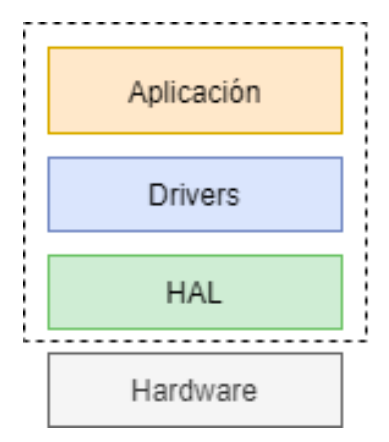
\includegraphics[width=0.2\linewidth]{Figuras/PatronCapas}
	\caption{}
	\label{fig:patroncapas}
\end{figure}


\subsubsection{Patrón Capa de abstracción de hardware (HAL)}
\begin{enumerate}
	\item Este patrón se utilizará para abstraer el acceso al hardware.
	\item Por definir debido a que no se a establecido el microcontrolador a emplear.
\end{enumerate}

\subsubsection{Observar y reaccionar}
\begin{enumerate}
	\item Este patrón se utiliza cuando un conjunto de sensores se monitorean y despliegan de manera rutinaria. Será utilizado para la arquitectura principal del software
	\item Se empleará este patrón arquitectónico para la capa aplicación.
\end{enumerate}

% TODO: \usepackage{graphicx} required
\begin{figure}[bph!]
	\centering
	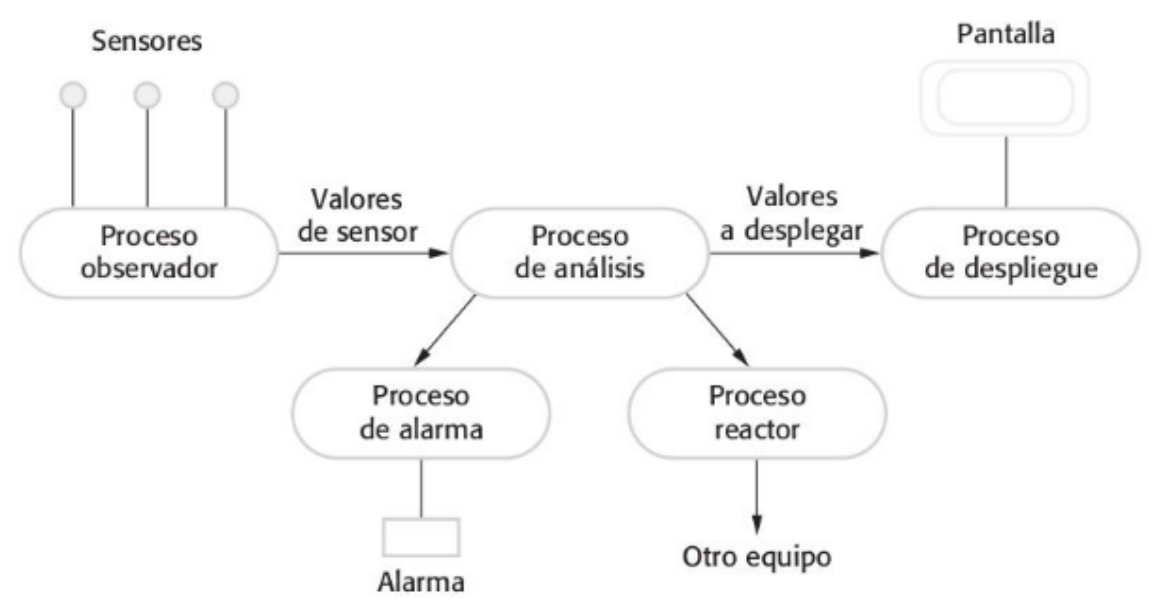
\includegraphics[width=0.7\linewidth]{Figuras/PatronObservarReaccionar}
	\caption{Patrón arquitectónico: “Observar y reaccionar” Imagen obtenida de diapositiva de la materia Ingeniería de Software.}
	\label{fig:patronobservarreaccionar}
\end{figure}


\subsubsection{Segmentación de procesos}
\begin{enumerate}
\item Este patrón se usa al transformar datos de una representación a otra antes de que puedan procesarse. Se implementa en la lectura de los sensores y en el proceso de comunicación con el servidor.
\item Se empleará este patrón arquitectónico para la capa aplicación.
\end{enumerate}

% TODO: \usepackage{graphicx} required
\begin{figure}[bph!]
	\centering
	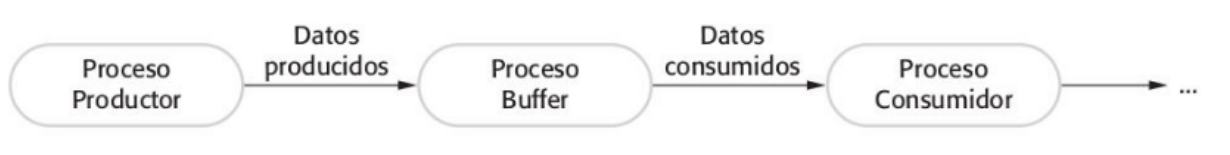
\includegraphics[width=0.9\linewidth]{Figuras/PatronSegmentacionProcesos}
	\caption{ Patrón arquitectónico: “Segmentación de procesos” Imagen obtenida de diapositiva de la materia Ingeniería de Software.}
	\label{fig:patronsegmentacionprocesos}
\end{figure}




\newpage

\subsection{Subsistemas}

En el desarrollo de nuestro sistema de monitoreo de calidad del aire, hemos estructurado el software en varios subsistemas interconectados, cada uno especializado en una función clave. Estos subsistemas incluyen Almacenamiento, Transmisión y Comunicación, Gestión de Energía, Interfaz de Usuario, Sincronización de Tiempo, y Seguridad y Resiliencia. Juntos, forman una arquitectura cohesiva que garantiza la eficiencia, precisión y fiabilidad del sistema en su conjunto, facilitando la recopilación, procesamiento y análisis de datos ambientales críticos."

Esta introducción proporciona un resumen claro y conciso de la estructura modular del software y su finalidad dentro del sistema global.





\begin{description}
	\item[Adquisición de datos:] este subsistema se encarga de la captura de datos en tiempo real utilizando sensores de MP2.5. Su función principal es recolectar datos sobre la concentración de partículas en el aire y su marca temporal para cada conjunto de datos. Estos datos serán enviados al subsistema de procesamiento para su análisis.
	
	\item[Procesamiento de datos:] responsable del procesamiento de los datos recogidos por los sensores. Incluye la realización de cálculos estadísticos, la estimación de la concentración promedio de MP2.5 y la generación de marcas temporales para cada conjunto de datos.
	
	\item[Almacenamiento:] gestiona el almacenamiento seguro y eficiente de los datos recogidos y procesados. Este subsistema asegura que toda la información relevante se conserve de manera organizada para su posterior acceso y análisis.
	
	\item[Transmisión y comunicación:] facilita la comunicación de datos entre el sistema de monitoreo y servidores externos o sistemas de gestión. Este subsistema es crucial para la transferencia de datos para análisis más profundos y para la integración con otras redes de monitoreo de calidad del aire.
	
	\item[Gestión de energía:] se encarga de proveer y gestionar la fuente de energía para todos los componentes del sistema. Asegura que el sistema funcione de manera continua y eficiente, y administra el consumo de energía.
	
	\item[Interfaz de usuario:] proporciona una plataforma para la interacción del usuario con el sistema. Puede incluir interfaces gráficas, paneles de control, y herramientas para configurar, operar y visualizar los datos recopilados por el sistema.
	
	\item[Sincronización de tiempo:] utiliza un Reloj de Tiempo Real (RTC) para asegurar que todas las mediciones estén correctamente sincronizadas y marcadas con la hora exacta. Esto es fundamental para análisis temporales y correlaciones de datos.
	
	\item[Seguridad y respuesta a fallos] Se enfoca en la protección de los datos y el sistema contra accesos no autorizados y fallos. Implementa medidas de seguridad y mecanismos de recuperación de errores para mantener la integridad y la disponibilidad de los datos.
\end{description}



\newpage

\subsection{Responsabilidades}
%2. Indicar brevemente qué responsabilidades tendrá cada subsistema y

La siguiente descripción corresponde a las responsabilidades que tendrá cada uno de los subsistemas de software \namesoftware. Desde la captura precisa de datos hasta la seguridad y resiliencia, cada subsistema cumple funciones críticas, asegurando la recopilación, procesamiento, almacenamiento y análisis de los datos.

\begin{description}
	\item[Adquisición de datos:] este bloque de software está diseñado para solicitar datos de los sensores de MP2,5 en intervalos regulares. La programación de estos intervalos es configurable, permitiendo adaptar el momento en que se toman las muestras. Además, el módulo tiene la responsabilidad de recoger datos del módulo de sincronización de tiempo, garantizando que cada lectura de MP2,5 de los sensores se vincule con una marca temporal exacta. Una vez recopilados, estos datos son enviados al subsistema de procesamiento. La estructura de la trama de datos generada se ajustará a un formato específico.
	
	\bigskip
	\begin{tabular}{|c|c|c|}
		\hline
		\textbf{ID SENSOR} &   \textbf{DIA HORA} & \textbf{CONCENTRACION MP2,5} \\
		\hline
		INT & AAAAMMDD HHMM & FLOAT \\
		\hline
	\end{tabular}

	\bigskip
	
	\item[Procesamiento de datos] Toma los datos generados por el bloque de adquisición y los dispone en una cola.  almacenados una cola de datos.  y se encarga de procesarlos. El procesamiento consiste en estimación  calcular la concentración promedio de MP2.5, y generar marcas temporales para cada medición.
	
	\item[Almacenamiento] Almacenar de forma segura las mediciones y los resultados del procesamiento para evitar la pérdida de datos.
	
	\item[Transmisión y comunicación] Enviar los datos procesados y almacenados a un servidor remoto o a otros sistemas para su análisis y monitoreo.
	
	\item[Gestión de energía] Asegurar un suministro de energía constante y eficiente para todos los componentes del sistema.
	
	\item[Interfaz de usuario] Permitir a los usuarios interactuar con el sistema, configurarlo y visualizar datos en tiempo real o históricos.
	
	\item[Sincronización de tiempo] Modulo encargado de proveer bajo demanda una referencia de tiempo precisa para las mediciones y los registros de datos.
	
	
	
	\item[Seguridad y respuesta a fallos] Proteger los datos y el sistema contra accesos no autorizados, errores y fallos, garantizando la integridad y disponibilidad de los datos.
\end{description}


\subsection{Interfaces externas y componentes}
 A continuación se indican los componentes externo e interfaces con sensores, actuadores y componentes que tendrá cada uno de los subsistemas:
	\begin{description}
		\item[Adquisición de datos:] Softa Sensores de MP2.5 para la captura de datos ambientales. [CND]
		\item[Procesamiento de datos:] Microcontrolador para el procesamiento de datos, software de cálculo estadístico. [CND]
		\item[Almacenamiento:] Memoria o dispositivos de almacenamiento de datos, como discos duros o sistemas en la nube. [CND]
		\item[Transmisión y comunicación:] Módulos de comunicación (como placa Wi-Fi, Ethernet, o GSM) para la transmisión de datos a servidor externo y señal a indicador led en el gabinete.
		\item[Gestión de energía:] Fuentes de alimentación, sistemas de gestión de energía (modulo transformador), y conexiones a la red eléctrica.[CND]
		\item[Interfaz de usuario:] Interfaces de usuario como led, paneles de control, interfaces web, y aplicaciones móviles [CND].
		\item[Sincronización de tiempo:] RTC (Reloj de Tiempo Real) para sincronizar las mediciones de tiempo. [CND]
		\item[Seguridad y resiliencia:] Sistemas de seguridad cibernética, mecanismos de autenticación, y software de recuperación de errores.[CND]
	\end{description}
	
\end{document}